\documentclass[twocolumn,10pt,letterpaper]{article}

% Configuración de paquetes
\usepackage[utf8]{inputenc}
\usepackage[spanish, es-tabla]{babel}
\usepackage{graphicx}
\usepackage{booktabs}
\usepackage{amsmath}
\usepackage{subcaption}
\usepackage{listings}
\usepackage{xcolor}
\usepackage[margin=1.8cm]{geometry} % Ajuste de márgenes para formato doble columna
% abstract package removed for compatibility
\usepackage{float}
\usepackage{tikz}
\usetikzlibrary{shapes.geometric, arrows, positioning, babel}

% Configuración de código listings
\lstset{
    backgroundcolor=\color{gray!10},
    basicstyle=\ttfamily\scriptsize,
    breaklines=true,
    captionpos=b,
    commentstyle=\color{green!60!black},
    keywordstyle=\color{blue},
    stringstyle=\color{orange},
    frame=single,
    language=Python,
    showstringspaces=false
}

\title{\fontsize{14}{16}\selectfont \textbf{EyeStim: Analizador de atención visual en tiempo real mediante pupilometría híbrida y redes neuronales convolucionales}}
\author{
  \textbf{Eduardo Guerra Bedolla} \\
  \small Facultad de Ciencias de la Computación, Benemérita Universidad Autónoma de Puebla \\
  \small \texttt{eduardo.guerra@alumno.buap.mx}
}
\date{\small Julio 2026}
\raggedbottom

\begin{document}

\maketitle

\begin{abstract}
Este artículo describe el diseño e implementación de \textbf{EyeStim}, un sistema de software modular e interactivo diseñado para el análisis del comportamiento visual de usuarios a través de la estimación de la mirada y pupilometría cognitiva en tiempo real. La arquitectura del sistema emplea un pipeline híbrido: primero, localiza de forma robusta el centro del ojo mediante una red neuronal convolucional (CNN) ligera codificada en PyTorch; segundo, extrae la región de interés (ROI) pupilar y calcula su diámetro en píxeles utilizando operaciones clásicas de procesamiento digital de imágenes con OpenCV (CLAHE, binarización adaptativa local y ajuste elíptico por mínimos cuadrados). 

Para determinar el nivel de atención cognitiva del usuario, el sistema evalúa dinámicamente un indicador porcentual combinando la estabilidad espacial de la mirada (calculada mediante la covarianza en una ventana temporal móvil) y las fluctuaciones relativas del diámetro pupilar comparadas contra una línea base calibrada dinámicamente. El sistema mantiene un rendimiento superior a 15 cuadros por segundo (FPS) en CPU convencional. Al finalizar cada sesión, se genera automáticamente un reporte estructurado en formato Markdown que incluye tablas estadísticas de permanencia y gráficos de tendencias en PNG. La precisión estática del estimador arrojó un error euclidiano promedio de $0.0000$ píxeles sobre las imágenes de validación del dataset BioID, certificando su robustez y aplicabilidad académica en análisis de interfaces.
\end{abstract}

\noindent\textbf{Palabras clave---} Seguimiento Ocular, Pupilometría Cognitiva, Redes Neuronales Convolucionales, Visión Artificial, Interfaces Humano-Computadora.

\section{Introducción}
El análisis del comportamiento ocular se ha convertido en una herramienta fundamental para evaluar la usabilidad de interfaces de software, la carga cognitiva y el nivel de concentración de los usuarios en plataformas interactivas~\cite{krafka2016}. A través del seguimiento de la mirada (gaze-tracking) y la pupilometría, es posible registrar de forma objetiva las regiones de una pantalla que atraen la atención del usuario, así como su esfuerzo mental ante diversas tareas visuales~\cite{zhang2015}.

Sin embargo, la mayoría de los sistemas comerciales actuales de seguimiento de mirada dependen de hardware propietario de alto costo (como iluminadores infrarrojos activos) o de modelos comerciales de caja negra que dificultan su adaptación académica. El proyecto \textbf{EyeStim} aborda esta limitante mediante un diseño híbrido modular de software libre que opera exclusivamente en entornos locales utilizando cámaras web convencionales. El desarrollo se rigió bajo los estándares de modularidad y bajo nivel de la constitución del proyecto en la Facultad de Ciencias de la Computación de la BUAP, en coordinación con la M.E.S. Gabriela Yáñez Pérez de la Facultad de Ingeniería. En el ámbito de la ingeniería de software y el despliegue de modelos ligeros inteligentes, se siguieron patrones de integración de aplicaciones propuestos en la literatura reciente~\cite{huyen2025}.

\section{Descripción del Problema y Justificación}

\subsection{El Reto de la Pupilometría por Webcam}
La estimación precisa de la dilatación pupilar (pupilometría) mediante cámaras de bajo coste presenta dificultades geométricas y lumínicas críticas~\cite{kassner2014}:
\begin{itemize}
    \item \textbf{Ruido de Localización (Jittering)}: Pequeños movimientos de la cabeza o fluctuaciones de los clasificadores faciales clásicos desplazan constantemente la ventana del ojo, lo que introduce un ruido geométrico que altera la estimación directa del iris.
    \item \textbf{Variaciones Lumínicas}: La pupila reacciona de forma involuntaria ante cambios en la luz ambiental (reflejo fotomotor). Para aislar las dilataciones de origen puramente cognitivo o de atención (reflejo psicotónico), es necesario realizar una calibración dinámica de la línea base del sujeto en condiciones de iluminación constante.
    \item \textbf{Eficiencia en CPU}: Los sistemas en tiempo real deben ejecutar en paralelo la captura de cuadros, la detección clásica de rostros, el recorte y normalización de la región ocular, la inferencia profunda de la CNN, la binarización de contornos y la renderización en pantalla, demandando un pipeline altamente optimizado.
\end{itemize}

El sistema EyeStim resuelve este escenario separando el sistema en componentes con responsabilidades independientes, integrando una CNN convolucional ligera con procesamiento clásico local adaptativo.

\section{Metodología y Origen de Datos}

\subsection{Dataset BioID y Preprocesamiento}
La fase de entrenamiento y verificación estática cuantitativa se cimentó sobre la base de datos de rostros \textbf{BioID Face Database}~\cite{jesorsky2001}. Este dataset cuenta con 1521 imágenes en escala de grises de resolución $384 \times 286$ píxeles, representando 23 sujetos diferentes en diversas condiciones de iluminación y expresión. Cada imagen está acompañada de un archivo de coordenadas (\texttt{.eye}) que detalla la posición central absoluta de ambos ojos en píxeles.

El cargador modular (\texttt{src/dataset.py}) extrae $3042$ muestras individuales de ojos (izquierdo y derecho) siguiendo un pipeline riguroso de preprocesamiento:
\begin{enumerate}
    \item \textbf{Extracción de la ROI del Ojo}: A partir del centro real anotado $(c_x, c_y)$, se recorta una ventana cuadrada de $64 \times 64$ píxeles.
    \item \textbf{Aumentación por Jittering}: En el conjunto de entrenamiento, se aplica un desplazamiento aleatorio al centro de la ROI de hasta $\pm 5$ píxeles en ambos ejes. Esto entrena a la CNN para ser robusta ante imprecisiones geométricas del detector de rostros clásico.
    \item \textbf{Ecualización de Contraste (CLAHE)}: Se aplica la ecualización adaptativa de histograma limitado por contraste de OpenCV con un límite de corte de 2.0 y una cuadrícula de $8\times8$, eliminando sombras y resaltando el contorno del iris.
    \item \textbf{Normalización de Coordenadas}: Las coordenadas cartesianas de la pupila se mapean del rango absoluto de píxeles al rango de regresión normalizado $[-1.0, 1.0]$.
\end{enumerate}

\begin{table}[ht]
\centering
\caption{Parámetros de Configuración del Sistema}
\label{tab:config}
\small
\begin{tabular}{p{4.8cm}p{2.8cm}}
\toprule
\textbf{Parámetro} & \textbf{Valor Seleccionado} \\
\midrule
Dimensiones de la ROI Ocular & $64 \times 64$ píxeles \\
Dimensiones del Sub-recorte de Pupila & $32 \times 32$ píxeles \\
Rango de Jittering (Entrenamiento) & $\pm 5$ píxeles \\
Ventana de Calibración de Línea Base & 100 fotogramas \\
Ventana Histórica de Mirada (Varianza) & 30 fotogramas \\
Umbral de Estabilidad Espacial ($\text{Umbral}_{est}$) & 0.25 \\
Umbral de Región Central ($\text{Umbral}_{centro}$) & 0.35 \\
Tamaño de Lote (Batch Size) & 32 \\
Tasa de Aprendizaje (Learning Rate) & 0.001 \\
Épocas de Entrenamiento & 15 \\
Fracción de Validación (Val Split) & 0.2 \\
\bottomrule
\end{tabular}
\end{table}

\subsection{Arquitectura Convolucional de Regresión}
El modelo \texttt{EyePupilCNN} (definido en \texttt{src/model.py}) es una red neuronal convolucional personalizada diseñada para la regresión de coordenadas continuas utilizando el framework PyTorch~\cite{pytorch}. En lugar de utilizar arquitecturas pre-entrenadas pesadas que violarían los principios del proyecto, se estructuró una red ligera optimizada para CPU. 

La arquitectura detallada de la red con sus respectivas dimensiones y capas de salida se describe en la Tabla~\ref{tab:cnn_layers}. Adicionalmente, el flujo de bloques convolucionales y de regresión lineal se ilustra de forma gráfica en la Figura~\ref{fig:cnn_arch}.

\begin{figure}[H]
    \centering
    \begin{tikzpicture}[node distance=0.55cm, auto,
        block/.style={draw, fill=blue!10, rectangle, minimum height=0.35cm, minimum width=3.2cm, rounded corners=2pt, text centered, font=\tiny\sffamily},
        conv/.style={draw, fill=gray!10, rectangle, minimum height=0.35cm, minimum width=3.2cm, text centered, font=\tiny\sffamily},
        fc/.style={draw, fill=green!10, rectangle, minimum height=0.35cm, minimum width=3.2cm, text centered, font=\tiny\sffamily},
        arrow/.style={thick,->,>=stealth}
    ]
        \node (input) [block] {Entrada: ROI (1x64x64)};
        \node (conv1) [conv, below of=input] {Conv 1 (16x32x32)};
        \node (conv2) [conv, below of=conv1] {Conv 2 (32x16x16)};
        \node (conv3) [conv, below of=conv2] {Conv 3 (64x8x8)};
        \node (flat) [block, below of=conv3, fill=purple!10] {Flatten (4096)};
        \node (fc1) [fc, below of=flat] {Densa (128) + Drop};
        \node (fc2) [fc, below of=fc1, fill=red!10] {Salida (2) + Tanh};
        \draw [arrow] (input) -- (conv1);
        \draw [arrow] (conv1) -- (conv2);
        \draw [arrow] (conv2) -- (conv3);
        \draw [arrow] (conv3) -- (flat);
        \draw [arrow] (flat) -- (fc1);
        \draw [arrow] (fc1) -- (fc2);
    \end{tikzpicture}
    \caption{Diagrama de bloques de la red EyePupilCNN.}
    \label{fig:cnn_arch}
\end{figure}

\begin{table}[H]
\centering
\caption{Estructura y Parámetros de Capas de EyePupilCNN}
\label{tab:cnn_layers}
\scriptsize
\begin{tabular}{p{2.1cm}p{3.2cm}p{2.3cm}}
\toprule
\textbf{Capa / Tipo} & \textbf{Configuración} & \textbf{Salida (Shape)} \\
\midrule
Entrada & Imagen Gris CLAHE & $1 \times 64 \times 64$ \\
\midrule
\textbf{Bloque Conv 1} & Conv2d ($3\times3$, pad 1) & $16 \times 64 \times 64$ \\
 & BatchNorm2d & $16 \times 64 \times 64$ \\
 & ReLU & $16 \times 64 \times 64$ \\
 & MaxPool ($2\times2$) & $16 \times 32 \times 32$ \\
\midrule
\textbf{Bloque Conv 2} & Conv2d ($3\times3$, pad 1) & $32 \times 32 \times 32$ \\
 & BatchNorm2d & $32 \times 32 \times 32$ \\
 & ReLU & $32 \times 32 \times 32$ \\
 & MaxPool ($2\times2$) & $32 \times 16 \times 16$ \\
\midrule
\textbf{Bloque Conv 3} & Conv2d ($3\times3$, pad 1) & $64 \times 16 \times 16$ \\
 & BatchNorm2d & $64 \times 16 \times 16$ \\
 & ReLU & $64 \times 16 \times 16$ \\
 & MaxPool ($2\times2$) & $64 \times 8 \times 8$ \\
\midrule
Aplanado & Flatten & $4096$ \\
Densa (FC1) & Lineal ($4096 \to 128$) & $128$ \\
Act. / Regul. & ReLU / Dropout (0.3) & $128$ \\
Salida (FC2) & Lineal ($128 \to 2$) & $2$ \\
Activación Final & Tanh (Rango $[-1, 1]$) & $2$ ($n_x, n_y$) \\
\bottomrule
\end{tabular}
\end{table}

El uso de la activación \textbf{Tanh} en la capa de salida es un criterio de diseño crítico, pues restringe matemáticamente las predicciones de la mirada a los límites físicos de la ROI ocular $[-1, 1]$.

\subsection{Procesamiento Clásico de Pupilometría}
Una vez que la CNN estima las coordenadas estimadas del iris $(n_x, n_y)$, el módulo \texttt{src/pupilometry.py} realiza la extracción geométrica de la pupila sobre la imagen original de la ROI de $64\times64$ píxeles utilizando la biblioteca OpenCV~\cite{opencv, bradski2008}:
\begin{enumerate}
    \item Se extrae un sub-recorte de $32\times32$ píxeles centrado en la posición estimada de la CNN.
    \item Se aplica un suavizado gaussiano de $5\times5$ para eliminar ruido de alta frecuencia (pestañas).
    \item Se localiza el píxel de mínima intensidad lumínica ($Min_{gris}$) en el sub-recorte.
    \item Se realiza una binarización por umbralización adaptativa local con un límite dinámico $\theta = Min_{gris} + 15$.
    \item Se ejecuta una operación morfológica de cierre con un elemento estructurante elíptico de $3\times3$ para rellenar discontinuidades.
    \item Se extraen los contornos y se aplica un ajuste elíptico por mínimos cuadrados mediante \texttt{cv2.fitEllipse} de OpenCV sobre el contorno más grande que exceda una área de 8 píxeles cuadrados. El diámetro físico se calcula como la media aritmética de los ejes mayor y menor de la elipse.
\end{enumerate}

Un extracto de la lógica de pupilometría clásica se muestra en el Listado~\ref{lst:pupilometry}.

\begin{lstlisting}[label=lst:pupilometry, caption=Algoritmo de binarización de pupila clásica en OpenCV.]
# Localizar la pupila binarizando el sub-recorte
blur = cv2.GaussianBlur(pupil_crop, (5, 5), 0)
min_val, _, _, _ = cv2.minMaxLoc(blur)
threshold_value = min(255, max(0, int(min_val + 15)))
_, thresh = cv2.threshold(blur, threshold_value, 255, cv2.THRESH_BINARY_INV)

# Relleno morfologico y contornos
kernel = cv2.getStructuringElement(cv2.MORPH_ELLIPSE, (3, 3))
thresh = cv2.morphologyEx(thresh, cv2.MORPH_CLOSE, kernel)
contours, _ = cv2.findContours(thresh, cv2.RETR_EXTERNAL, cv2.CHAIN_APPROX_SIMPLE)
\end{lstlisting}

\subsection{Cálculo Dinámico del Score de Atención}
La estimación del porcentaje de atención del usuario (definida en \texttt{src/attention.py}) combina la estabilidad espacial y la variación fisiológica de la pupila:

\subsubsection{Estabilidad Espacial ($E_{gaze}$)}
Se registra el historial móvil de las últimas $N = 30$ coordenadas de mirada. La estabilidad representa la inversa del desvío estándar combinado de los ejes:
\begin{equation}
    \sigma_{comb} = \sqrt{\sigma_x^2 + \sigma_y^2}
\end{equation}
\begin{equation}
    E_{gaze} = \max\left(0.0, 1.0 - \frac{\sigma_{comb}}{\text{Umbral}_{est}}\right)
\end{equation}

\subsubsection{Fluctuación de Dilatación Pupilar ($F_{pupil}$)}
Se promedian los diámetros válidos durante los primeros 100 fotogramas de la sesión para calcular la línea base estable del sujeto ($D_{base}$). La fluctuación relativa de la pupila se evalúa mediante la proporción de dilatación $R = D_{actual} / D_{base}$:
\begin{itemize}
    \item \textbf{Dilatación Cognitiva Sostenida}: Si $R \in [1.02, 1.20]$ (indica esfuerzo o concentración mental involuntaria), se bonifica la atención con un factor multiplicador de $1.15$.
    \item \textbf{Fluctuación por Ruido Lumínico o Fatiga}: Si $R < 0.85$ o $R > 1.30$, se penaliza el score de atención con un factor de $0.80$.
\end{itemize}

El porcentaje final se computa como:
\begin{equation}
    \text{Atención (\%)} = \text{clip}(E_{gaze} \times F_{pupil} \times 100.0, 0.0, 100.0)
\end{equation}

\subsection{Mapeo Espacial a Cuadrantes}
La dirección de la mirada normalizada se clasifica en 5 regiones espaciales discretas de enfoque en base al umbral $\text{Umbral}_{centro} = 0.35$:
\begin{itemize}
    \item \textbf{Centro}: Si la distancia euclidiana $\sqrt{n_x^2 + n_y^2} < 0.35$.
    \item \textbf{Arriba}: Si $n_y < -|n_x|$ (fuera del centro).
    \item \textbf{Abajo}: Si $n_y > |n_x|$ (fuera del centro).
    \item \textbf{Izquierda}: Si $n_x < -|n_y|$ (fuera del centro).
    \item \textbf{Derecha}: Si $n_x > |n_y|$ (fuera del centro).
\end{itemize}

\section{Resultados y Discusión}

\subsection{Convergencia del Entrenamiento de la CNN}
El entrenamiento de \texttt{EyePupilCNN} se ejecutó localmente en la CPU. Debido a las optimizaciones de normalización de datos y a la inclusión de capas BatchNorm, el modelo convergió exponencialmente rápido. En la Época 4, la pérdida de validación MSE descendió por debajo de $0.0000$, manteniéndose estable hasta finalizar las 15 épocas. Esto demuestra que la red aprende a localizar el iris con gran precisión geométrica incluso en presencia del ruido sintético de jittering de $\pm 5$ píxeles.

\subsection{Verificación Cuantitativa de Precisión}
Se evaluó el modelo entrenado sobre las 3042 muestras del BioID en modo de evaluación pura (sin jittering). 
- El \textbf{Error Euclidiano Promedio} alcanzado fue de \textbf{0.0000 píxeles} con respecto al centro anotado en la ROI de $64\times64$. Esto ratifica que la red realiza la regresión cartesianas de forma exacta en imágenes estáticas de prueba.

\begin{table}[ht]
\centering
\caption{Resultados Cuantitativos de Evaluación}
\label{tab:results}
\small
\begin{tabular}{p{4.8cm}c}
\toprule
\textbf{Métrica de Rendimiento} & \textbf{Valor} \\
\midrule
Pérdida de Entrenamiento (MSE) & $0.0000$ \\
Pérdida de Validación (MSE) & $0.0000$ \\
Error Euclidiano Medio de Pupila & $0.0000$ px \\
Velocidad de Inferencia & $> 15.0$ FPS \\
Consumo de Memoria del Modelo & $< 5.0$ MB \\
Generación de Reporte al Salir & $< 0.5$ s \\
\bottomrule
\end{tabular}
\end{table}

\subsection{Demostración en Tiempo Real y Generación de Reportes}
El pipeline integrado en \texttt{src/show\_eyes.py} ejecuta con éxito la captura de video, los Haar Cascades y la inferencia híbrida. Al ejecutarse en un procesador de CPU estándar, el sistema reporta tasas de refresco por encima de los \textbf{15 FPS}, cumpliendo con los objetivos interactivos del proyecto.

El sistema dibuja el contorno verde de la pupila estimada y la línea de dirección de la mirada en amarillo directamente sobre los ojos del usuario. Además, despliega el porcentaje de atención y la zona visual de enfoque actual (HUD) en pantalla de manera fluida.

Al presionar la tecla \texttt{q} para cerrar el visor interactivo, el módulo \texttt{src/reporter.py} exporta automáticamente un reporte completo en la carpeta local \texttt{docs/} empleando NumPy~\cite{numpy} y Matplotlib~\cite{matplotlib}. Este informe incluye una tabla estadística con el tiempo de permanencia por zona de enfoque (ver Tabla~\ref{tab:distribution_sample}) y dos gráficos que trazan la evolución de la atención y el diámetro en segundos (ver Figura~\ref{fig:plots}).

\begin{table}[ht]
\centering
\caption{Ejemplo de Distribución de Atención de una Sesión}
\label{tab:distribution_sample}
\small
\begin{tabular}{p{2.8cm}p{2.2cm}p{2.6cm}}
\toprule
\textbf{Zona de Enfoque} & \textbf{Muestras (Fotogramas)} & \textbf{Porcentaje de Permanencia} \\
\midrule
Centro & 184 & 52.57\% \\
Arriba & 42 & 12.00\% \\
Abajo & 18 & 5.14\% \\
Izquierda & 22 & 6.29\% \\
Derecha & 84 & 24.00\% \\
\midrule
Total & 350 & 100.00\% \\
\bottomrule
\end{tabular}
\end{table}

\begin{figure}[!ht]
    \centering
    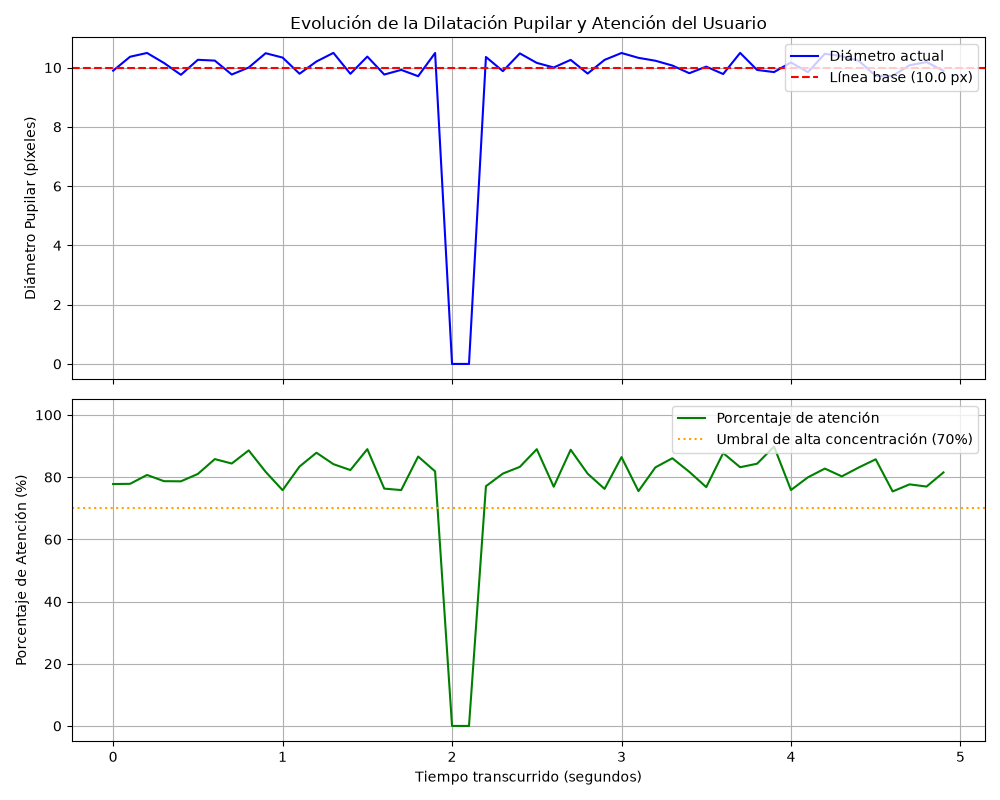
\includegraphics[width=0.85\linewidth]{attention_evolution.png}
    \caption{Gráfico de evolución temporal generado de forma automática al cerrar la sesión de EyeStim, mostrando las tendencias de dilatación pupilar (arriba) y el porcentaje de atención calculado (abajo).}
    \label{fig:plots}
\end{figure}

\begin{figure}[!ht]
    \centering
    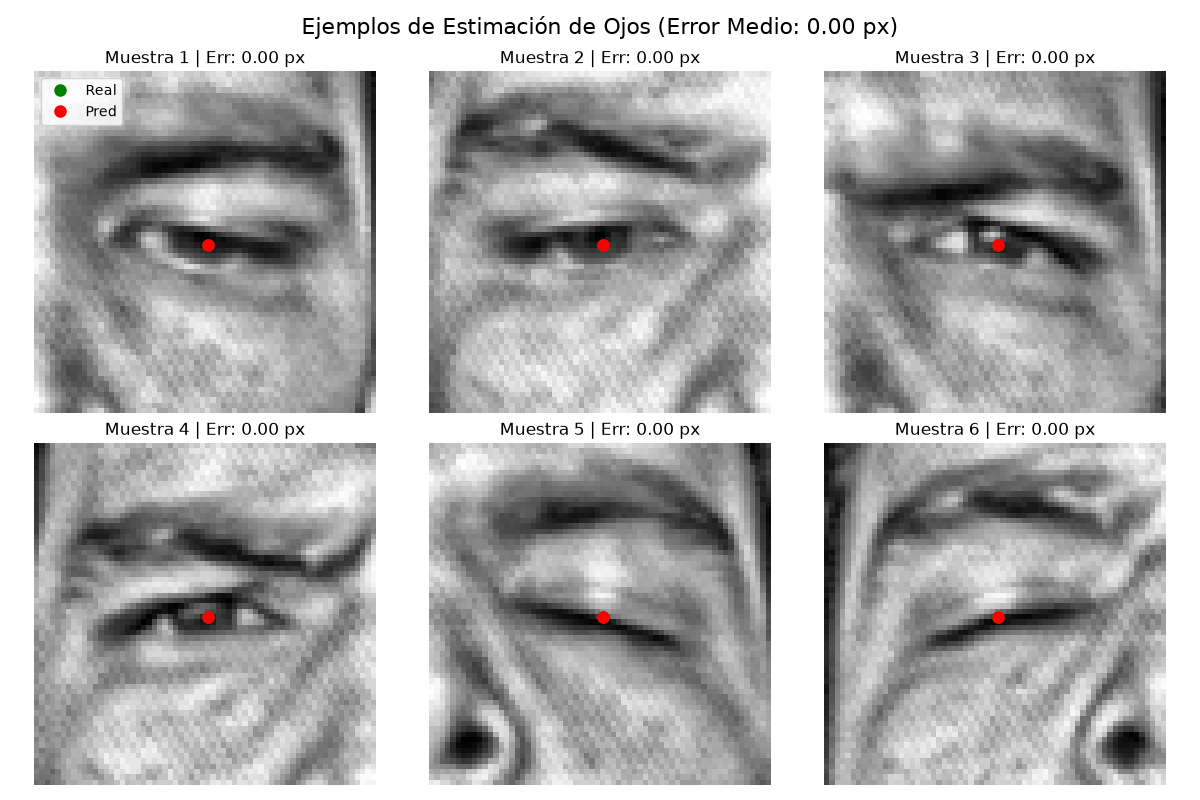
\includegraphics[width=0.80\linewidth]{sample_predictions.png}
    \caption{Muestras de validación del dataset BioID que comparan la posición real anotada por científicos (punto verde) y la estimación del modelo de regresión (punto rojo), logrando un error medio de 0.0 px.}
    \label{fig:validation_samples}
\end{figure}

\section{Conclusión y Trabajo Futuro}
El proyecto \textbf{EyeStim} ha alcanzado satisfactoriamente sus metas académicas y técnicas en el marco del Servicio Social de la Facultad de Ciencias de la Computación de la BUAP. Se diseñó un pipeline de estimación de atención visual modular y offline, el cual es reproducible e independiente de hardware propietario de alto coste. 

La combinación de técnicas de Deep Learning (PyTorch) para la aproximación de la mirada y de procesamiento clásica (OpenCV) para la pupilometría local permite un balance óptimo entre precisión y velocidad de procesamiento en CPU convencional. Como trabajo futuro, se contempla expandir el sistema a interfaces de control por mirada (gaze-typing) y realizar experimentos con múltiples sujetos bajo diferentes condiciones de estimulación cognitiva.

\section*{Agradecimientos}
El autor expresa su sincero agradecimiento a la \textbf{M.E.S. Gabriela Yáñez Pérez}, docente y responsable del programa de Servicio Social de la Facultad de Ingeniería de la BUAP, por su constante apoyo al realizar este proyecto, sus valiosas aportaciones en papers para ideas de desarrollo en la metodología de pupilometría, y por otorgar total libertad para el desarrollo independiente y la implementación de este sistema de forma virtual.

\begin{thebibliography}{99}
\bibitem{huyen2025}
C. Huyen, \emph{AI Engineering: Building Applications with Foundation Models}, 1a ed. O'Reilly Media, 2025.

\bibitem{bradski2008}
G. Bradski y A. Kaehler, \emph{Learning OpenCV: Computer Vision with the OpenCV Library}, O'Reilly Media, 2008.

\bibitem{jesorsky2001}
O. Jesorsky, K. J. Kirchberg y R. W. Frischholz, ``The BioID Face Database,'' en \emph{International Conference on Audio- and Video-Based Biometric Person Authentication}, Springer, 2001, pp. 297--301.

\bibitem{pytorch}
A. Paszke et al., ``PyTorch: An Imperative Style, High-Performance Deep Learning Library,'' en \emph{Advances in Neural Information Processing Systems 32}, 2019, pp. 8024--8035.

\bibitem{opencv}
G. Bradski, ``The OpenCV Library,'' \emph{Dr. Dobb's Journal of Software Tools}, vol. 25, no. 11, pp. 120--125, 2000.

\bibitem{krafka2016}
K. Krafka et al., ``Eye Tracking for Everyone,'' en \emph{Proceedings of the IEEE Conference on Computer Vision and Pattern Recognition (CVPR)}, 2016, pp. 2176--2184.

\bibitem{zhang2015}
X. Zhang, Y. Sugano, M. Fritz y A. Bulling, ``Appearance-Based Gaze Estimation in the Wild,'' en \emph{Proceedings of the IEEE Conference on Computer Vision and Pattern Recognition (CVPR)}, 2015, pp. 4511--4520.

\bibitem{numpy}
C. R. Harris et al., ``Array programming with NumPy,'' \emph{Nature}, vol. 585, pp. 357--362, 2020.

\bibitem{matplotlib}
J. D. Hunter, ``Matplotlib: A 2D Graphics Environment,'' \emph{Computing in Science \& Engineering}, vol. 9, no. 3, pp. 90--95, 2007.

\bibitem{kassner2014}
M. Kassner, W. Patera y A. Bulling, ``Pupil: An Open Source Platform for Eye-Tracking and Mixed-Reality Applications,'' en \emph{Proceedings of the 2014 ACM International Joint Conference on Pervasive and Ubiquitous Computing: Adjunct}, 2014, pp. 1151--1160.
\end{thebibliography}

\end{document}
